\chapter{The Sparsest cut problem}

Same as before we have an undirected graph $G = (V,E)$ and $k$-pairs of sources and targets $(s_{1},t_{1}), (s_{2}, t_{2}), \dots, (s_{k}, t_{k}) \in V^{2}$. But we will introduce a new parameters $d_{1}, d_{2}, \dots, d_{k} \in \R^{+}$ called \textbf{demands}.

Firstly we will take a look at linear program for solving this problem for $k = 1$.

$$
\begin{aligned}
	\max f \\
	\sum_{p \in \mathcal{P}_{st}} x_{p} \geq f \cdot d_{1} \\
	\sum_{e \in \in \mathcal{P}_{st}} x_{p} \leq c(e) & \quad \forall e \in E\\
	x \geq 0
\end{aligned}
$$

Where $\mathcal{P}_{st}$ are all paths between $s$ and $t$. We may see that the optimum of the max flow is the same as this optimum just divided by $d_{1}$. We will denote $\mathcal{P}_{i} = \mathcal{P}_{s_{i}, t_{i}}$.

\section{Concurrent multicommodity flow}

Thus we are getting this LP for all $k$ commodities and $k$ demands.

$$
\begin{aligned}
	\max f \\
	\sum_{p \in \mathcal{P}_{i}} x_{p} \geq f \cdot d_{i} & \quad \forall i \in [k]\\
	\sum_{i = 0}^{k} \sum_{e \in \in \mathcal{P}_{i}} x_{p} \leq c(e) & \quad \forall e \in E\\
	x \geq 0
\end{aligned}
$$

We will take a look at the matrix of this LP and after that find a dual program. But firstly we modify $\sum_{p \in \mathcal{P}_{i}} x_{p} \geq f \cdot d_{i}$ to $f \cdot d_{i} - \sum_{p \in \mathcal{P}_{i}} x_{p} \leq 0$. Then the matrix is as follows:

$$
\begin{matrix}
	  & f     &    & \mathcal{P}_{1} &       &    & \mathcal{P}_{2} &       & \dots \\
	1 & d_{1} & -1 & -1              & \dots &  0 & \dots           & 0     & \dots \\
	2 & d_{2} & 0  &  0              & \dots & -1 & -1              & \dots & 0     \\
	\vdots  \\
	k & d_{k} & 0  &  0              & \dots & 0 & 0               &  0    & \dots \\
	e_{1} & 0     & 1  &  0              &       & 1 & 0               &  0    & \dots \\
	\vdots \\
	e_{|E|} & 0     & 0  &  1              &       & 1 & 0               &  1    & \dots \\
\end{matrix}
$$

Where for the first $k$ lines are $\leq 0$ and for edges it is $\leq c(e)$. We visualized the matrix and thus we can make the dual. We will have variables $x_{e}$ for edges and $y_{i}$ for $i \in [k]$. Thus the dual is:

$$
\begin{aligned}
	\min \sum_{e \in E} x_{e}c(e) \\
	\sum_{i = 0}^{k} y_{i}d_{i} \geq 1 \\
	\sum_{e \in p} x_{e} -y_{i} \geq 0 & \quad \forall i \in [k] \forall p \in \mathcal{P}_{i}\\
	x,y \geq 0
\end{aligned}
$$

\begin{defn}
	For $S \subseteq V$ we define $\delta(S) = \{\{u,v\} \in E : |\{u,v\} \cap S| = 1\}$ and then $I(S) = \{i \in [k] : |\{s_{i}, t_{i}\} \cap S| = 1\}$. Then the \textbf{sparsity} of $S$ is
	
	$$
	\rho(S) = \frac{\sum_{e \in \delta(S)}c(e)}{\sum_{i \in I(S)} d_{i}}
	$$
\end{defn}

\begin{example}
	We will have a simple example where all capacities are 1 and all demands are 1. So we have the graph \ref{example-sparse}.
	
	\begin{figure}[!h]\centering
		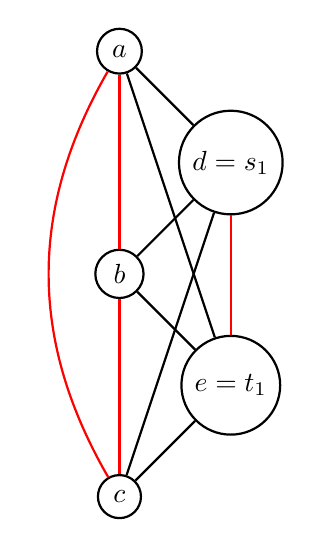
\begin{tikzpicture}[node distance={20mm}, thick, main/.style = {draw, circle}]
			\node[main] (1) {$a$};
			\node[main] (2) [below right of=1] {$d = s_{1}$};
			\node[main] (3) [below left of=2] {$b$};
			\node[main] (4) [below right of=3] {$e = t_{1}$};
			\node[main] (5) [below left of=4] {$c$};
			\draw (1) -- (2);
			\draw (1) -- (4);
			\draw (3) -- (2);
			\draw (3) -- (4);
			\draw (5) -- (2);
			\draw (5) -- (4);
			\draw [red] (1) -- (3);
			\draw [red] (5) -- (3);
			\draw [red] (2) -- (4);
			\path (1) edge [bend right, red] (5);
		\end{tikzpicture}
		\label{example-sparse}
		\caption{Sparse cut example.}
	\end{figure}
	
	The demands are the red edges. We may see that if we choose $S = \{c, e\}$ then $\sum_{e \in \delta(S)} c(e) = 3$ and $\sum_{i \in I(S)} d_{i} = 3$ therefore $\rho(S) = 1$.
	
	We may see that each pair $s_{i}$ $t_{i}$ consumes at least 2 units of a flow of the network for a single unit of the flow. Then we set $f$ as a max flow and see what we get. For example for paths $\mathcal{P}_{1} = \{(d,a,e) = p_{1}, (d,b,e) = p_{2}, (d,c,e) = p_{3}\}$. $x_{p_{1}} + x_{p_{2}} + x_{p_{3}} \geq f \cdot d-{1} = f$. Thus the total volume consumed by a flow with objective value $f$ is $\geq k 2 f = 8f$. Total volume of $G$ is 6. Therefore $f \leq \frac{6}{8} = \frac{3}{4}$.
	
	Maybe we can ask if there exist such a flow with this volume. We can obtain it by pushing $\frac{1}{4}$ from $d$ to $c$ on each path and $\frac{3}{8}$ between all other pairs on all paths. All edges are not over their capacities and we get $\frac{3}{4}$ for all demands.
\end{example}

\begin{defn}
	Now $F \subseteq E : I(F) = \{i \in [k] : s_{i}, t_{i} \text{ are in different components in } (V, E \setminus F)\}$. And \textbf{sparsity} of $F$ be
	
	$$
	\rho(F) = \frac{\sum_{e \in F}c(e)}{\sum_{i \in I(F)} d_{i}}
	$$
\end{defn}

\begin{lemma}
	$\min_{S \subseteq V} \rho(S) = \min_{F \subseteq E} \rho(E)$.
\end{lemma}

\begin{proof}
	The $\geq$ inequality can be easily seen if we set $F$ to be $\delta(S)$. Now we need to show the other inequality. For given $F \subseteq E$, let $s_{1}, \dots s_{l}$ be the components of connectivity of $(V, E \setminus F)$. For that we will proof that $\min_{i \in [l]} \rho(s_{i}) \leq \rho(F)$. This will bw shown by a contradiction. Assume $\forall i$:
	
	$$
	\begin{aligned}
		\frac{\sum_{e \in \delta(s_{i})}c(e)}{\sum_{j \in I(s_{i})} d_{j}} &> \frac{\sum_{e \in F}c(e)}{\sum_{j \in I(F)} d_{j}}\\
		\sum_{e \in \delta(s_{i})}c(e) &> \rho(F) \cdot \sum_{j \in I(s_{i})} d_{j}
	\end{aligned}
	$$
	
	Now we sum all $i$ inequalities.
	
	$$
	\sum_{i = 1}^{l} \sum_{e \in \delta(s_{i})}c(e) > \rho(F) \cdot \sum_{i = 1}^{l} \sum_{j \in I(s_{i})} d_{j}
	$$

	We can see that $\sum_{i = 1}^{l} \sum_{e \in \delta(s_{i})}c(e) = 2 \sum_{e \in F} c(e)$ because all edges are counted twice and similarly $\sum_{i = 1}^{l} \sum_{j \in I(s_{i})} d_{j} = 2 \sum_{j \in I(F)} d_{j}$. So we get:
	
	$$
	\sum_{e \in F} c(e) > \rho(F) \cdot \sum_{j \in I(F)} d_{j}
	$$
	
	Which is a contradiction. So for each $F$ we can find $s_{i}$ that satisfies the inequality.
\end{proof}

Now we can use this for integer program and then use relaxation. The program will look like this:

$$
\begin{aligned}
	\min \frac{\sum_{e \in E} c(e) x_{e}}{\sum_{i = 1}^{k}d_{i}y_{i}} \\
	\sum_{e \in p} x_{e} \geq y_{i} & \quad \forall i \in [k] \forall p \in \mathcal{P}_{i}\\
	\sum_{i = 1}^{k} d_{i}y_{i} \geq 1 \\
	x_{e} \in \{0,1\} &\quad \forall e \in E\\
	y_{i} \in \{0,1\} &\quad \forall i \in [k]
\end{aligned}
$$

At least one edge has to be removed from each path. Plus we assume that $d_{i} \geq 1$. Now we could just put $x_{e} \geq 0$ and $y_{i} \geq 0$. But the thing is that we don't have a linear function in the objective function. What if we have a vector $(x,y) \to (\alpha x, \alpha y)$ for $\alpha > 0$. You can see that the feasible solution don't change and also the objective is the same. So we could put $\alpha = \frac{1}{\sum_{i = 1}^{k} d_{i}y_{i}}$ and we know that the $\sum_{i = 1}^{k} d_{i}y_{i} = 1$. Thus the linear program will be:

$$
\begin{aligned}
	\min \sum_{e \in E} c(e) x_{e} \\
	\sum_{e \in p} x_{e} \geq y_{i} &\quad \forall i \in [k] \forall p \in \mathcal{P}_{i}\\
	\sum_{i = 1}^{k} d_{i}y_{i} = 1 \\
	x_{e} \geq 0 &\quad \forall e \in E\\
	 y_{i} \geq 0 &\quad \forall i \in [k]
\end{aligned}
$$

Before we continue we remind ourselves the Manhattan distance $||z||_{1} = \sum_{j=1}^{k} |z_{j}|$. This is indeed a metric, which means that it is non-negative, symmetric and triangular inequality holds.

\begin{lemma}
	Let $f$ be a mapping $f: V \to \R^{d}$ for some $d > 0$ and let
	
	$$
	\begin{array}{r r c l}
		\forall \{u,v\} \in E: & \hat{x}(\{u,v\}) & = & ||f(u) - f(v)||_{1} \\
		\forall i \in [k]: & \hat{y}(i) & = & ||f(s_{i}) - f(t_{i})||_{1} \\
		& \beta & = & \sum_{i = 1}^{k} d(i) \hat{y}(i).
	\end{array}
	$$
	
	Then $\left(\frac{\hat{x}}{\beta}, \frac{\hat{y}}{\beta}\right)$ is feasible solution. Also this is called \textbf{solution induced by $f$}. And we will denote $\left(\frac{\hat{x}}{\beta}, \frac{\hat{y}}{\beta}\right) = \left(x', y'\right)$.
\end{lemma}

\begin{proof}
	We need to show that all conditions of LP are satisfied. Easily the non-negativity still holds. Also
	
	$$
	\sum_{i=1}^{k} y'(i) d(i) = \sum_{i=1}^{k} \frac{\hat{y}(i)}{\beta}d(i) = 1
	$$
	
	where the last equality holds by the definition of $\beta$. Lastly we need to check that $\sum_{e \in E} x(e) \geq y(i)$ of our LP still holds. This can be easily proven by the fact that $||\cdot||_{1}$ is metric so in particular triangular inequality is satisfied and by induction on the length of the path we would prove it. Also keep in mind that scaling by $\beta$ doesn't change anything for the whole inequality since it is on both sides.
\end{proof}

\begin{lemma}[A]\label{A}
	Let $(x',y')$ be a solution induced by $f : V \to \R^{d}$. Then one can find in polynomial time cut $S \subseteq V$ of sparsity $\rho(S) \leq \sum_{e \in E} x'(e) c(e)$.
\end{lemma}

\begin{lemma}[B]\label{B}
	Given any feasible solution $(x,y)$ of LP, one can construct a mapping $f: V \to \R^{d}$ (by random algorithm with high probability) which induces a solution $(\bar{x}, \bar{y})$ s.t.
	
	$$
	\sum_{e \in E} c(e) \bar{x}(e) = O(\log k) \sum_{e \in E} c(e) x(e)
	$$
\end{lemma}

\begin{thm}
	There exist a randomized polynomial-time algorithm for the sparsest cut problem that is $O(\log k)$-approximation.
\end{thm}

\begin{proof}
	By Lemma B (\ref{B}) we generate $(\bar{x}, \bar{y})$ and then by Lemma A (\ref{A}) we construct the cut.
\end{proof}

\begin{proof}[Proof of Lemma A \ref{A}]
	Given $f: V \to \R^{d}$ let
	
	$$
	\begin{array}{l r c l}
		\forall u,v \in V & \mu (u,v) & = & ||f(u) - f(v)||_{1}
	\end{array}
	$$
	
	For $S \subseteq V$ we define $\forall u,v \in V$
	
	$$
	\mu_{S}(u,v) =
	\left\{
	\begin{array}{l l}
		1 & \text{iff } |\{u,v\} \cap S| = 1 \\
		0 & \text{otherwise}
	\end{array}
	\right.
	$$
	
	This will be called \textbf{cut mapping} and we can easily see that it is non-negative, symmetric and triangular inequality is satisfied thus it is metric. Before we continue we will use another lemma.
	
	\begin{lemma}[lemma]\label{lemma}
		$\forall S \subseteq V \ \exists \lambda_{S} \geq 0$ s.t. $\forall u,v \in V: \mu(u,v) = \sum_{S \subseteq V} \lambda_{S} \mu_{S}(u,v)$. Moreover $|\{S | \lambda_{S} > 0\}| \leq n \cdot d$.
	\end{lemma}
	
	\begin{proof}[Proof of lemma \ref{lemma}]
		Consider the contribution of the first coordinate to $\mu(u,v)$: order the vertices according to $f_{1}$ where $f = (f_{1}, f_{2}, \dots, f_{d})$, s.t. $f_{1}(v_{1}) \leq f_{1}(v_{2}) \leq \dots \leq f_{1}v_{n}$. Now let $S(l) = \{v_{1}, \dots, v_{l}\}$ for $l \in [n]$. Consider any two vertices $v_{i},v_{j}$ s.t. $i > j$.
		
		$$
		f_{1}(v_{i}) - f_{1}(v_{j}) = \sum_{l=j}^{i-1} (f_{1}(v_{l+1}) - f_{1}(v_{l})) = \sum_{l = 1}^{n-1} (f_{1}(v_{l+1}) - f_{1}(v_{l})) \mu_{S(l)} (v_{i}, v_{j}) 
		$$
		
		Where $(f_{1}(v_{l+1}) - f_{1}(v_{l})) = \lambda_{S(l)}$. This can be used to prove this for all dimensions $f_{2}, \dots, f_{d}$ thus it is true for $f$.
	\end{proof}
	
	\begin{observ}
		For any non-negative numbers $a_{1}, \dots, a_{n}$ and positive numbers $b_{1}, \dots, b_{n}$ holds:
		
		$$
		\frac{\sum_{i = 1}^{n} a_{i}}{\sum_{i = 1}^{n} b_{i}} \geq \min_{i \in [n]} \frac{a_{i}}{b_{i}}
		$$
	\end{observ}
	
	\begin{proof}[Proof of observation]
		By a contradiciton assume $\forall j:$
		
		$$
		\begin{aligned}
			\frac{\sum_{i = 1}^{n} a_{i}}{\sum_{i = 1}^{n} b_{i}} &< \frac{a_{j}}{b_{j}}\\
			b_{j} \frac{\sum_{i = 1}^{n} a_{i}}{\sum_{i = 1}^{n} b_{i}} &< a_{j}\\
			\sum_{j} b_{j} \frac{\sum_{i = 1}^{n} a_{i}}{\sum_{i = 1}^{n} b_{i}} &< \sum_{j} a_{j}
		\end{aligned}
		$$
		
		Where the last line is summing all the inequalities together. We get a contradiction. \textit{Note that geometricaly that can be represent as vectors and values of the $\tan$ function and it would state that there is a $\tan$ smaller of one of the vectors than the sum of them.}
	\end{proof}
	
	Now we continue to proof the Lemma A.
	
	$$
	\sum_{e \in E} c(e) x'(e) = \frac{\sum_{e \in E}c(e) x'(e))}{\sum_{i = 1}^{k}y'(i) d(i)}
	$$
	
	Which is just a division by $1$ from the conditions in LP. Then by lemma:
	
	$$
	\begin{aligned}
		& = \frac{\sum_{e \in E} c(e) \sum_{S \subseteq V} \lambda_{S} \mu_{S}(e)}{\sum_{i =1}^{k} d(i) \sum_{S \subseteq V} \lambda_{S} \mu_{S}(s_{i},t_{i})}\\
		&= \frac{\sum_{S \subseteq V} \lambda_{S} \sum_{e \in E} c(e) \mu_{S}(e)}{\sum_{S \subseteq V} \lambda_{S} \sum_{i =1}^{k} d(i)  \mu_{S}(s_{i},t_{i})}\\
		&\geq \min_{S \subseteq V} \rho(S)
	\end{aligned}
	$$
	
	The last part is due to the previous observation and the fact that $\sum_{e \in E} c(e) \mu_{S}(e) = a_{S}$ and $\sum_{i =1}^{k} d(i)  \mu_{S}(s_{i},t_{i}) = b_{S}$ taken means $\frac{a_{S}}{b_{S}} = \rho(S)$.
\end{proof}

Now we will be proving the Lemma A \ref{B}. For that we denote $T = \{s_{i} | i \in [k]\} \cap \{t_{i}| i \in [k]\}$ and without loss of generality assume that $|T| = 2^{\tau}$ (we can add arbitrary sources and targets that are essentially the same). Let us denote $d_{x} (u,v)$ the length of the $x$-shortest $u-v$ path. Where $x$ is the result of our LP. For $A \subseteq V: d_{x}(A,u) = \min_{v \in A} d_{x}(v,u)$.

Also we put $L = q \log (k)$ where $q$ is some constant to be decided later on and $k$ is for number of commodities. Also $d = L \cdot \tau = O (\log^{2}(k))$. For $t = 1, \dots, \tau$ and $l = 1, \dots, L$: let $A_{tl}$ be a set that is constructed by $2^{\tau - t}$-times selecting uniformely at random $v \in V$.

\begin{defn}
	$\forall v \in V: f_{tl}(v) = d_{x}(v, A_{tl})$.
\end{defn}

\textit{Note that both $A_{tl}$ and $f_{tl}$ are not dependent on $l$. One can say that $l$ is for repeating the selection.}

\begin{lemma}
	$\forall \{u,v\} \in E : || f(u) - f(v)||_{1} \leq d \cdot x(u,v)$.
\end{lemma}

\begin{proof}
	We proceed by the definition and some algebra.
	
	$$
	|| f(u) - f(v)||_{1} = \sum_{t = 1}^{\tau} \sum_{l = 1}^{L} |f_{tl}(u) - f_{tl}(v)| = \sum_{t = 1}^{\tau} \sum_{l = 1}^{L} |d_{x}(u, A_{tl}) - d_{x}(v, A_{tl})|
	$$
	
	Now lets take a look at these inequalities which follows from the triangle inequalities.
	
	$$
	\begin{array}{r c l}
		d_{x}(u, A_{tl}) & \leq & x(u,v) + d_{x}(v, A_{tl}) \\
		d_{x}(v, A_{tl}) & \leq & x(u,v) + d_{x}(u, A_{tl}) \\
		& \Downarrow & \\
		d_{x}(u, A_{tl}) - d_{x}(v,A_{tl}) & \leq & x(u,v) \\
		d_{x}(v, A_{tl}) - d_{x}(u,A_{tl}) & \leq & x(v,u)
	\end{array}
	$$
	
	Which leads to $|d_{x}(u,A_{tl}) - d_{x}(v, A_{tl})| \leq x(u,v)$ and thus getting the last inequality:
	
	$$
	\sum_{t = 1}^{\tau} \sum_{l = 1}^{L} |d_{x}(u, A_{tl}) - d_{x}(v, A_{tl})| \leq \tau \cdot L \cdot x(u,v) = d \cdot x(u,v)
	$$
\end{proof}

\begin{lemma}
	With probability $\geq 1/2$: $\forall i \in [k]$ holds that
	
	$$
	||f(s_{i}) - f(t_{i})||_{1} \geq \frac{L}{88} y_{i}.
	$$
\end{lemma}

Before proving this lemma we will take a look, how useful it is. $\beta = \sum_{i = 1}^{k} d(i) \cdot ||f(s_{i}) - f(t_{i})||_{1} = \Omega(\log k) \cdot \sum_{i = 1}^{k} d(i) y_{i} = \Omega(\log k)$ where $y_{i}$ is from our LP and thus $\sum_{i = 1}^{k} d(i) y_{i}$ is equal to 1. The second equality is from the lemma before. And now from the lemma even before that we get $\leq \sum_{e \in E} c(e) \cdot d \cdot x(e) = d \sum_{e \in E} c(e) x(e)$ which is the objective function result of our LP. Thus $= O(\log^{2}(k)) \sum_{e \in E} x(e) c(e)$. But that is scaled by $\beta$ thus the objective value of the solution induced by $f$ is $\leq O(\frac{\log^{2}(k)}{\log(k)} \sum_{e \in E} c(e) x(e) = O(\log k) \sum_{e \in E} x(e) c(e)$ and so we have $O(\log k)$-approximation. So this proves the Lemma B \ref{B}.

\begin{proof}
	To prove the lemma we will prove a simple version that for fixed $i \in [k]$ with probability $\geq 1 - 1/2k$ it holds that
	
	$$
	||f(s_{i}) - f(t_{i})||_{1} \geq \frac{L}{88} y_{i}.
	$$
	
	We can easily see that for doing this for all $i \in [k]$ the lemma will follow. To prove this we will define few more things.
	
	$$
	\begin{aligned}
		\forall v \in \{s_{i}, t_{i}\}: &\ B_{x}(v, r) = \{w \in T | d_{x}(v,w) \leq r\}\\
		\forall v \in \{s_{i}, t_{i}\}: &\ B_{x}^{\circ}(v, r) = \{w \in T | d_{x}(v,w) < r\}
	\end{aligned}
	$$
	
	Now we will look at this sequence of radii. $r_{0} = 0$,
	
	$$
	r_{t} = \min \{r > 0 : |B_{x}(s_{i},r)| \geq 2^{t} \land |B_{x}(t_{i},r)| \geq 2^{t}\}
	$$
	
	$$
	\hat{t} = \min \left\{t | r_{t} \geq \frac{y(i)}{4}\right\}
	$$
	
	and also redefine $r_{\hat{t}} = \frac{y(i)}{4}$. This is define with respect to LP. And also it means that $B_{x}(s_{i}, r_{\hat{t}}) \cap B_{x}(t_{i}, r_{\hat{t}}) = \emptyset$.
	
	Now we observe that for $A_{tl} \subseteq V:$ $A_{tl} \cap B_{x}^{\circ}(s_{i}, r_{t}) = \emptyset \Leftrightarrow d_{x}(s_{i}, A_{tl}) \geq r_{t}$. And also $A_{tl} \cap B_{x}(t_{i}, r_{t - 1}) \neq \emptyset \Leftrightarrow d_{x}(t_{i}, A_{tl}) \leq r_{t - 1}$. Let $E_{tl}$ be the event such that $A \cap B = \emptyset$ and $A \cap G \neq \emptyset$ where $B = B_{x}^{\circ}(s_{i}, r_{t})$ and $G = B_{x}(t_{i}, r_{t - 1})$.
	
	We may observe that if $E_{tl}$ happens then $|f_{tl}(s_{i}) - f_{tl}(t_{i})| = |d_{x}(s_{i}, A_{tl}) - d_{x}(t_{i}, A_{tl})| \geq r_{t} - r_{t -1}$. We will look at the  probability of happening this.
	
	$$
	\begin{aligned}
		\Pr[E_{tl}] & = \Pr[A_{tl} \cap G \neq \emptyset | A_{tl} \cap B = \emptyset] \Pr[A_{tl} \cap B = \emptyset] \\
		            & \geq \Pr[A_{tl} \cap G \neq \emptyset] \Pr[A_{tl} \cap B = \emptyset]
	\end{aligned}
	$$
	
	Let us assume wlog $s_{i}$ defines $r_{t}$.
	
	$$
	\Pr[A_{tl} \cap B = \emptyset] = \left( 1 - \frac{|B|}{|V|} \right) ^{2^{\tau - t}} \geq \left( 1 - \frac{2^{t}}{2^{\tau}} \right) ^{\frac{2^{\tau}}{2^{t}}} \geq \frac{1}{e} \geq \frac{1}{4}
	$$
	
	$$
	\Pr[A_{tl} \cap G \neq \emptyset] = (1 - \Pr[A_{tl} \cap G = \emptyset]) = 1 - \left( 1 - \frac{|G|}{|V|} \right)^{2^{\tau - t}} \geq
	$$
	
	$$
	\geq 1 - \left( 1 - \frac{2^{t -1}}{2^{\tau}} \right)^{\frac{2^{\tau}}{2^{t-1}} \frac{1}{2}} \geq 1 - \left( \frac{1}{e} \right)^{\frac{1}{2}} \geq \frac{4}{11}
	$$
	
	Thus the $\Pr[E_{tl}] \geq \frac{1}{11}$. Now we fix $t = \{1, \dots, \tau\}$ and define:
	
	$$
	X_{tl} = \left\{
	\begin{array}{l l}
		1 & \text{ iff } E_{tl} \text{ occurs} \\
		0 & \text{otherwise}
	\end{array}
	\right.
	$$
	
	For $l = 1, \dots, L$ let $\mu = \E \left[ \sum_{l = 1}^{L} X_{tl} \right]$. We may observe that $\mu \geq \frac{L}{11}$ by linearity of $\E$. We now may use the Chernoff bound.
	
	$$
	\Pr \left[ \sum_{l = 1}^{L} X_{tl} \leq \frac{\mu}{2} \right] \leq e^{\frac{-\mu}{8}} \leq e^{\frac{-q \log k}{88}} \leq e^{-\log 2k - \log\log2k} = \frac{1}{2k \log 2k}
	$$
	
	Where there is hidden analysis to proper choice of $q$. If $\sum_{l = 1}^{L} X_{tl} \geq \frac{\mu}{2}$ then
	
	$$
	\sum_{l = 1}^{L} |f_{tl}(s_{i}) - f_{tl}(t_{i})| \geq \sum_{l = 1}^{L} X_{tl} (r_{t} - r_{t-1}) \geq \frac{L}{22} (r_{t} - r_{t-1})
	$$
	
	Therefore with probability $\geq 1 - \frac{\tau}{2k \log 2k} \geq 1 - \frac{1}{2k}$ $\forall t \in [\hat{t}]$ the previous statement holds. Thus
	
	$$
	||f(s_{i}) - f(t_{i})||_{1} \geq \frac{L}{88} y_{i} = \frac{L}{88} 4 \sum_{t = 1}^{\tau} (y_{t} - y_{t-1})
	$$
\end{proof}

\section{Metric spaces}

Some of basic definitions are for metric spaces which reader may already know, but we will remind it once again.

\begin{defn}
	Metric space $(M,d)$ when $d : M \times M \to \mathbb{R}^{+}$ and
	
	\begin{enumerate}[(i)]
		\item $\forall x,y \in M: d(x,y) \geq 0$ and $d(x,y) = 0 \Leftrightarrow x = y$,
		\item $\forall x,y \in M : d(x,y) = d(y,x)$,
		\item $\forall x,y,z \in M: d(x,z) \leq d(x,y) + d(y,z)$.
	\end{enumerate}
\end{defn}

We may already know some examples. One is for $G = (V,E)$ and for $x : E \to \mathbb{R}^{+}$ the metric is $d(z,y) = \min_{z-y \text{ paths}} \sum_{e \in P} x(e)$. This means that $(V,d)$ is a metric system.

\begin{defn}
	Let $(X,d)$ and $(Y,\bar{y})$ be metric spaces. An injective function $f : X \to Y$ is $D$-embedding for some $D \geq 1$, if $\exists r > 0$ such that $\forall x,y \in X$ the following holds
	
	$$
	r \cdot d(x,y) \leq \bar{d}(f(x), f(y)) \leq D \cdot r \cdot d(x,y).
	$$
\end{defn}

\begin{defn}
	The $\inf$ of $D$ values satisfying the above property is called \textbf{distortion} of $f$.
\end{defn}

\begin{thm}[Bourgain, 1985]
	Every $n$-point metric space $(V,d)$ can be embedded in $(\mathbb{R}^{p}, l_{1})$ with distortion $O(\log n)$ with $p = O(\log ^{2} n)$. Where $l_{1} = ||x||_{1} = \sum_{i}x_{i}$.
\end{thm}

We remind ourselves what we did. We constructed $f : V \to \mathbb{R}^{+}$ and $p = O(\log^{2} k)$ such that

\begin{enumerate}[(i)]
	\item $\forall u,v \in V : ||f(u) - f(v)||_{1} \leq p \cdot d_{x}(u,v)$,
	\item $\forall i \in [k] : ||f(s_{i}) - f(t_{i})||_{1} \geq \Omega(\log k) d_{x}(s_{i}, t_{i})$.
\end{enumerate}

So if we take $T = V$, think about all pair of vertices as commodities. Everything in the proof still works. So we technically proved this theorem before.

Now the question one can ask is: \textit{Is the analysis tight?} For the answer we may recall that in 3-regular graphs, there are $\Omega (n^{2})$ pairs of vertices at distance $\Omega (\log k)$. That was for the multi-commodity system. Lets consider 3-regular $\beta$-expanders (i.e. $\delta (S) \geq \beta|S|, \forall S \subseteq V, |S| \leq |V|/2$).

With that consider the instance: Commodity for each pair of vertices and set all $d = 1$. This will lead to

$$
\min_{S \subseteq V} \frac{E(S, V \setminus S)}{I(S)} \geq \min_{S \subseteq V} \frac{\beta |S|}{|S| |V \setminus S|} \geq \frac{\beta}{|V|} = \Omega(1/n)
$$

then the max concurrent flow is at most the available capacity $O(n)$ divided by what unit of flow consumes. Thus get

$$
\frac{O(n)}{\Omega (n^{2} \log n)} = O\left( \frac{1}{n \log n} \right)
$$

which means that it is tight. Alternatively integrality gap of our LP is $\Omega(\log n)$. Also it implies that the asymptotic optimality of the theorem is tight. Otherwise if there was better version we could use that for better approximation of our LP which is a contradiction. Also there exists $O(\sqrt{\log n})$-approximation for sparsest cut using positive semidefinite programming.

\begin{cor}
	Max flow $\leq$ min cut $\leq O(\log k)$ max flow. For sparsest cut problem.
\end{cor}

\section{Applications}

\begin{defn}
	Cut $(S, V \setminus S)$ is $b$-balanced (for some $b \leq 1/2$) if
	
	$$
	b n \leq |S| \leq (1-b)n
	$$
	
	where $G = (V,E)$ and $|V| = n$.
\end{defn}

$1/2$-balanced is called \textbf{bisection}. Also there is a problem for finding a $b$-balanced cut minimizing the number of edge between $E(S, V \setminus S)$ (\textit{cost of cut}). This problem is generally NP-hard.

\begin{thm}
	If there is a $b$-balanced cut $T$ in $G = (V,E)$, then for any $b' < \min\{1/3, b\}$ one can find in polynomial time $b'$-balanced cut of cost $O \left(\frac{E(T, V \setminus T) \log n}{b-b'}\right)$.
\end{thm}

\begin{proof}
	First we define the algorithm.
	
	\begin{algorithm}
		\caption{Find $b'$-balanced cut.}
		\begin{algorithmic}[1]
			\Require Graph $G$.
			\Ensure $b'$-balanced cut.
			\State $i := 0$, $G_{i} = G$, $S = \emptyset$
			\While{$|V(G_{i})| > (1-b')|V| $}
			\State find an approximation of the sparsest cut in $G_{i}$ and denote it as $S_{i} \subseteq V(G_{i})$
			\State let $G_{i+1} = G_{i}[V(G_{i}) \setminus S_{i}]$, $S = S \cup S_{i}$, $i = i+1$
			\EndWhile
			\Return S
		\end{algorithmic}
	\end{algorithm}
	
	where in the sparsest cut problem is on the network where all vertices are terminals and demands are $1$.
	
	Correctness of the algorithm: Before the last iteration it is true that $|S| < b'n$. In the last iteration at most $|V(G_{i})| / 2$ are added to $S$. Therefore at the end
	
	$$
	\leq |S| + \frac{n - |S|}{2} = \frac{n + |S|}{2} < \frac{(1+ b')n}{2} \leq (1- b')n
	$$
	
	Where the last inequality is due the value $b' \leq 1/3$ and the fact that $1+b' \leq 2-2b'$. Also because it ended $|S| \geq b'n$ so it is indeed a $b'$-balanced cut.
	
	Approximation of the cost:	Consider an optimal $b$-balanced cut $(T, V \setminus T)$. In each iteration $|T \setminus S| \geq (b - b') n$. What is the sparsity of the cut $T \setminus S$? Lets denote $\text{opt} = E(T, V \setminus V)$. The sparsity is
	
	$$
	\leq \frac{\text{opt}}{b - b')n(1-b)n} \leq \frac{2 \text{opt}}{(b-b')n^{2}}
	$$
	
	so the sparsity of the $O(\log n)$-approximation $S_{i}$ found by the algorithm is
	
	$$
	\frac{E(S_{i}, V_{i} \setminus S_{i})}{|S_{i}| |V_{i} \setminus S_{i}|} \leq O(\log n) \frac{\text{opt}}{(b-b')n^{2}}
	$$
	
	which means that $E(S_{i}, V_{i} \setminus S_{i}) \leq O(\log n) \frac{\text{opt}}{(b-b')n^{2}} |S_{i}|$. Now we sum it up.
	
	$$
	E(S, V \setminus S) \leq \sum_{i} E(s_{i}, V_{i} \setminus S_{i}) \leq O(\log n) \frac{\text{opt}}{(b-b')n^{2}} \sum_{i} |S_{i}| = O(\log n) \frac{\text{opt}}{b - b'}
	$$
\end{proof}

\section{Minimum cut linear arrangement}

Given $G = (V,E)$, find ordering $v_1, \dots, v_n$ of the vertices such that

$$
\max_{i \subset [n]} E(\{v_{1}, \dots, v_{i}\}, \{v_{i}, \dots, v_{n}\}) \text{ is minimized.}
$$

\begin{observ}
	$OPT \geq \min$ bijection of $G = : \mathcal{B}$.
\end{observ}

\begin{proof}
	For any ordering $E(\{v_{1}, \dots, v_{n/2}\} \{v_{n/2 +1}, \dots, v_{n}\}) \geq B$.
\end{proof}

\begin{algorithm}
	\caption{Find minimum cut linear arrangement}
	\begin{algorithmic}[1]
		\Require{Graph $G$}
		\Ensure{Minimum cut linear arrangement}
		\State Find a $1/3$-balanced cut of $G$ and denote it as $(L,R)$ by the previous algorithm.
		\State Solve the problem recursively for $L,R$.
	\end{algorithmic}
\end{algorithm}

\begin{observ}
	The depth of recursion is $O(\log n)$.
\end{observ}

\begin{observ}
	$E(L,R) \leq O (\log n) \cdot B$.
\end{observ}

And now we would like to get similiar bound for all the levels of recursion. For that consider $G_{i}$. Lets denote $B_{i}$ the bijection of $G_{i}$ and $OPT_{i}$ the optimum solution for $G_{i}$. Then $B_{i} \leq OPT_{i} \leq OPT$, therefore in our solution

$$
\forall i \in [n], E(\{v_{1}, \dots, v_{i}\} \{v_{i+1}, \dots, v_{n}\}) \leq O(\log n) \cdot O(\log n) \cdot OPT
$$

because the first $O$ is for number of recursion calls and the second $O$ is approximation of the size of each balanced cut. Altogether it is equal to $O(\log^2 n) OPT$.

\begin{thm}
	The approximation ratio of the algorithm is $O(\log^2 n)$.
\end{thm}

\begin{defn}
	Crossing number of the graph is the number of intersections of edges (the minimum). For planar graphs it is 0 and for not planar it is $\geq 1$.
\end{defn}

This can be also solved by the algorithm above.